% vim: spell spelllang=en:
\documentclass[12pt, oneside]{article}
\usepackage[a4paper, left=2.5cm, right=2.5cm, top=2.5cm, bottom=2.5cm]{geometry}

\usepackage[utf8]{inputenc} % Use unicode
\usepackage[T1]{fontenc}
\usepackage[english]{babel} % Names in spanish

%% Bibliography:
%\usepackage{comment}
%\usepackage[
    %backend=biber,
    %style=numeric,
%]{biblatex}
%\DeclareNameAlias{default}{last-first}

%\usepackage{csquotes}       % For bibliography quotations
%\DeclareQuoteAlias{spanish}{catalan}

%\addbibresource{biblio.bib}
%% see:
%% https://www.sharelatex.com/learn/Bibliography_management_in_LaTeX#The_bibliography_file

%\usepackage{datetime} % Customize date
%% \monthyeardate\today gives the date without the day
%\newdateformat{monthyeardate}{%
    %\monthname[\THEMONTH], \THEYEAR}

% For cross references
\usepackage[colorlinks = true]{hyperref}
\usepackage[catalan]{varioref}
%\usepackage{cleveref}
%hyperref configuration so that it doesn't contrast so much colorlinks,
\hypersetup{
   linkcolor={black},
   citecolor={black},
   %linkcolor={red!50!black},
   %citecolor={blue!50!black},
   urlcolor={blue!80!black}
}

\usepackage{xcolor}     % color

\usepackage{mathtools}  % amsmath + more
\usepackage{amsthm}     % Theorem enviroment
\usepackage{amssymb}    % More symbols
\usepackage{amstext}    % Text inside mathenv

\usepackage{relsize}    % Bigger math with mathlarger{___}
\usepackage{nicefrac}   % nice fractions in one line

\usepackage[export]{adjustbox}  % Adjust table size
\usepackage{float}              % Force tables and images position (H and H!)
\usepackage{wrapfig}            % Wrap images like in HTML

\usepackage{tabularx, colortbl, booktabs}    % Better tables
\usepackage{longtable}                      % Multiple page table

% Split cell in lines and more formating options inside table
\usepackage{array, multirow, multicol, makecell}

%\usepackage{subcaption}                     % Subfigures
%\usepackage[framemethod=tikz]{mdframed}     % Custom frames

%\usepackage[bottom]{footmisc} % Footnotes at bottom of page

%\usepackage[alsoload=hep]{siunitx}          % SI units and uncertainties
%\sisetup{locale = FR}                       % Commas and so on for spanish
%\sisetup{separate-uncertainty=true}
%\sisetup{
  %per-mode=fraction,
  %fraction-function=\nicefrac
%}

%\usepackage{tikz}
%%\usetikzlibrary{arrows}
%%\usetikzlibrary{scopes}
%\usetikzlibrary{babel}

%\usepackage{listings}       % For code blocks

%% Custom code highlight
%\definecolor{codegreen}{rgb}{0,0.6,0}
%\definecolor{codegray}{rgb}{0.5,0.5,0.5}
%\definecolor{codepurple}{rgb}{0.58,0,0.82}
%\definecolor{backcolour}{rgb}{0.95,0.95,0.92}
%\definecolor{lightblue}{RGB}{135,206,250}

%\lstdefinestyle{mystyle}{ backgroundcolor=\color{backcolour},
    %commentstyle=\color{codegreen}, keywordstyle=\color{blue},
    %numberstyle=\tiny\color{codegray}, stringstyle=\color{red},
    %identifierstyle=\color{black}, basicstyle=\footnotesize,
    %%breakatwhitespace=false,
    %breaklines=true,
    %%captionpos=b,                    keepspaces=true,
    %numbers=left,                    numbersep=5pt,
    %showspaces=false,
    %%showstringspaces=false, showtabs=false,
    %tabsize=4
%}
%\lstset{style=mystyle}

\newcommand{\whitepage}{
    \clearpage\thispagestyle{empty}\addtocounter{page}{-1} \newpage \clearpage
}

% Add command before appendix session for page numbering: A-1
%\newcommand{\appendixpagenumbering}{
    %\break
    %\pagenumbering{arabic}
    %\renewcommand{\thepage}{\thesection-\arabic{page}}
%}

%% Custom Math operators (functions not in italic in math mode):
%\DeclareMathOperator{\arcsec}{arcsec}
%\DeclareMathOperator{\arccot}{arccot}
%\DeclareMathOperator{\arccsc}{arccsc}
%\DeclareMathOperator{\cis}{cis}


\usepackage[justification=centering]{caption}
\usepackage{subcaption}
\usepackage{graphicx}
\usepackage{enumitem}
\usepackage{lipsum}

\usepackage{siunitx}
\usepackage{hyphenat}

\usepackage{xcolor}

\definecolor{LightGray}{rgb}{0.83, 0.83, 0.83}
\definecolor{bg}{HTML}{282828}

\usepackage[newfloat]{minted}
\captionsetup[listing]{position=top}

\setminted{
style=monokai,
%frame=lines,
framesep=2mm,
baselinestretch=1.2,
breaklines,
bgcolor=bg,
fontsize=\footnotesize,
linenos
}

\renewcommand\theadfont{\bfseries}

\title{
    PAR Laboratory Assignment\\
    Lab 4: Divide and Conquer parallelism with OpenMP: Sorting
}

\author{
    par2109:
    Aleix Boné,
    Alex Herrero
}

\date{
    Spring 2019-20
}

\begin{document}

\thispagestyle{empty}
\clearpage
\setcounter{page}{-1}

\begin{titlepage}
{
    \centering
    \null
    \vfill
    {\Huge \bfseries PAR Laboratory Assignment\par}
    \vspace{3em}
    {\Large {\scshape Lab 4:} Divide and Conquer parallelism with OpenMP: Sorting \par}
    \vfill
\begin{center}
\end{center}
    \vspace{3cm}

    \vfill
    {\raggedleft \Large
        Aleix Boné\\
        Alex Herrero\\
        {\bfseries\ttfamily par2109}\\
        \vspace{4em}
        2020-05-15
        \par}
}
\end{titlepage}

\tableofcontents
\pagebreak

\section{Introduction}%
\label{sec:intro}

\subsection{Analysis with \emph{Tareador}}

\begin{listing}[H]
\inputminted[firstline=20,lastline=31]{c}{sources/multisort-tareador-leaf.c}
\inputminted[firstline=33,lastline=51]{c}{sources/multisort-tareador-leaf.c}
\caption{Calls to the tareador API added to multisort-tareador.c for the leaf task decomposition}
\label{listing:tareador_leaf}
\end{listing}

\begin{listing}[H]
\inputminted[firstline=20,lastline=31]{c}{sources/multisort-tareador-tree.c}
\inputminted[firstline=33,lastline=51]{c}{sources/multisort-tareador-tree.c}
\caption{Calls to the tareador API added to multisort-tareador.c for the tree task decomposition}
\label{listing:tareador_leaf}
\end{listing}

\begin{figure}[H]
\centering
%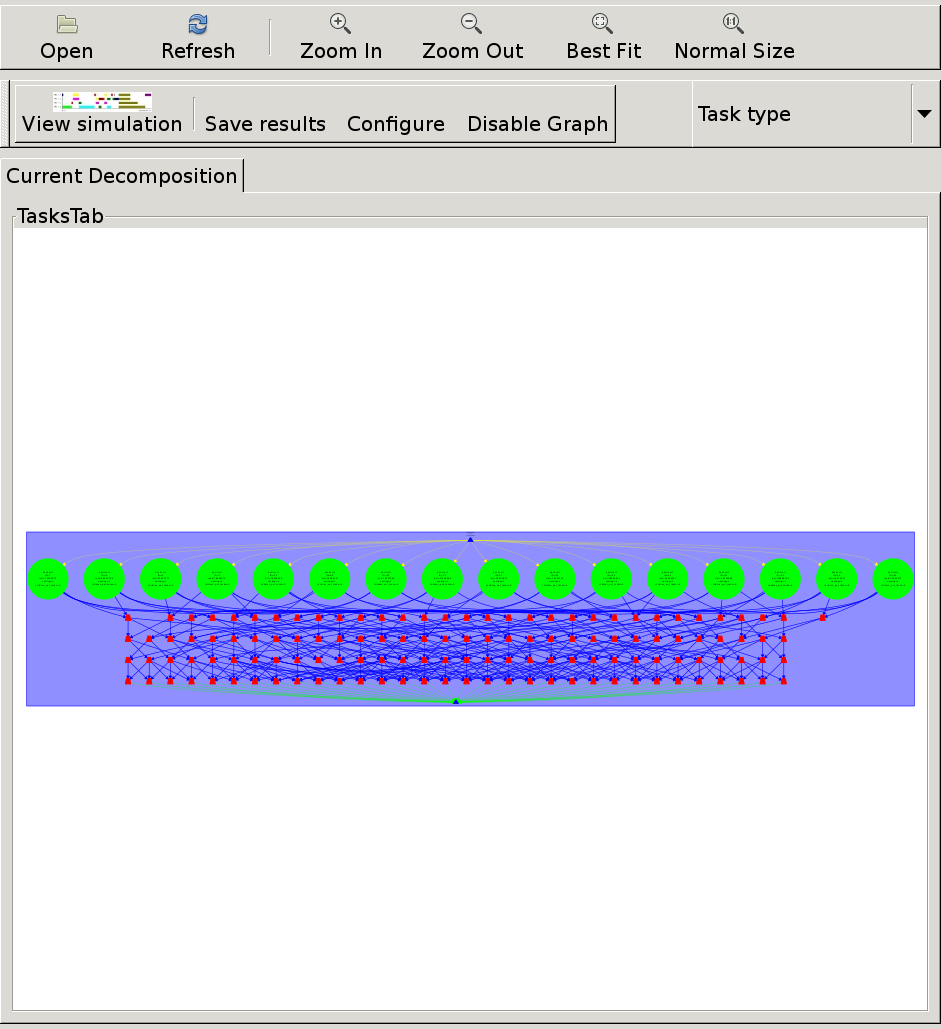
\includegraphics[width=0.8\textwidth]{captures/tareador-leaf.png}
\includegraphics[width=\textwidth]{dependency_graph_leaf.pdf}
\caption{Task graph for leaf decomposition}
\label{fig:tar_tasks_leaf}
\end{figure}

\begin{figure}[H]
\centering
\includegraphics[width=0.8\textwidth]{dependency_graph_tree.pdf}
\caption{Task graph for tree decomposition}
\label{fig:tar_tasks_tree}
\end{figure}

\begin{table}[H]
\centering
\begin{tabular}{lrrrrr}
\toprule
Leaf strategy & & & & & \\
\midrule
Recursion level:        & 1     & 2     & 3     & 4     & 5  \\
Num tasks generated:    & 16    & 32    & 32    & 32    & 32 \\
\bottomrule
\end{tabular}

\caption{Number of tasks that are generated at each recursion level for leaf strategy} 
\label{tab:Execution_time}
\end{table}

\begin{table}[H]
\centering
\begin{tabular}{lrrrrrrrrrrrrrrrrr}
\toprule
Tree strategy & & & & & & & & & & & & & & & & &\\
\midrule
Recursion level:        & 1     & 2     & 3     & 4     & 5     & 6     & 7     & 8     & 9     & 10    & 11    & 12    & 13    & 14    & 15    & 16    & 17  \\
Num tasks generated:    & 1     & 1     & 4     & 8     & 16    & 4     & 8     & 16    & 2     & 4     & 8     & 16    & 1     & 2     & 4     & 8    & 16 \\
\bottomrule
\end{tabular}

Leaf
Threads: 1 2 4 8 16 32 64
Execution time (ms): 1.263.350  631.688

Tree
Threads: 1 2 4 8 16 32 64
Execution time: 

\caption{Number of tasks that are generated at each recursion level for tree strategy} 
\label{tab:Execution_time}
\end{table}


\section{Parallelization strategies}%
\label{sec:par_strats}


\begin{listing}[H]
\inputminted[firstline=32,lastline=63]{c}{sources/multisort-omp-leaf.c}
\caption{OpenMP pragmas added for leaf decomposition}
\label{listing:omp_leaf}
\end{listing}

\begin{listing}[H]
\inputminted[firstline=32,lastline=74]{c}{sources/multisort-omp-tree.c}
\caption{OpenMP pragmas added for tree decomposition}
\label{listing:omp_tree}
\end{listing}

\begin{listing}[H]
\inputminted[firstline=32,lastline=74]{c}{sources/multisort-omp-tree-cutoff.c}
\caption{OpenMP pragmas added for tree decomposition with cutoff}
\label{listing:omp_tree_cutoff}
\end{listing}

\section{Performance evaluation}%
\label{sec:perf_eval}

\section{Conclusions}%
\label{sec:conclusions}

\end{document}
